\section{Evaluation Protocol}
\label{sec:experiments}

The evaluation covers prompted extraction, silver-supervised Qwen adaptation, and encoder initialization for Chinese competency extraction, with diagnostics by type, span length, and false positives on sentences without reference spans. The human reference set provides primary evaluation targets; supplementary silver validation and test scores measure agreement with generated annotations.

\subsection{Datasets and Splits}

The original corpus was partitioned by source document into training, development, and test sets with 1,600, 200, and 200 document identifiers, respectively. These partitions share no document identifiers and differ from the later labeled splits used for Silver supervision and human-reference evaluation.

We checked the Silver training and development sets for sentence-level overlap. JobBERT-zh + CRF uses Silver sets of 2,156 training and 169 development records. For Qwen and the encoder comparison, six training records matching three development texts after NFC normalization were removed, leaving 2,150 training and 169 development records. In this split, training and development share no identical or NFC-normalized complete texts, and neither contains a human-reference sentence by identifier or normalized text.

An audit of source-document identifiers found that the 2,150-record Silver training set shared one group with development and 59 groups with the human reference set. The latter contain 143 of the 150 reference sentences. These are different sentences from shared documents, which may contain multiple job postings. Reference sentences are excluded from supervised inputs, but their source documents overlap with training data.

Supplementary expanded-pool Qwen experiments use 8,842/348/350 training/validation/test records from the adopted expanded pool and 8,943/351/352 from the alternative pool. Both combine earlier supervision with additional annotations and differ in annotation channel and included records. Records shared across annotation-channel variants keep their split assignments. Checkpoints are selected by typed exact-span F1 on Silver validation labels. Silver-test scores measure agreement with generated labels in a separate sentence split whose source-document groups overlap with training. Sentence-level checks also excluded human-reference sentences from expanded-model fitting and checkpoint selection. Expanded-model settings and results appear in \hyperref[app:c]{Appendix~C}; duplicate records, normalization checks, and source-group overlaps appear in \hyperref[app:d]{Appendix~D}.

\subsection{Evaluation Metrics}

The primary metric is typed exact-span micro-F1: a match requires identical span boundaries and L/K/S/T type. Typed relaxed-span micro-F1 uses one-to-one greedy matching of same-type spans with intersection-over-union (IoU) of at least 0.5:

\begin{equation}
\mathrm{IoU}(u,v)=\frac{|u\cap v|}{|u\cup v|},
\qquad \mathrm{IoU}(u,v)\geq 0.5.
\label{eq:span-iou}
\end{equation}

Here, $u$ and $v$ are the sets of Unicode-code-point positions in the predicted and reference spans; $\lvert\cdot\rvert$ counts positions. Under either matching rule, true positives (TP) are matched prediction--reference pairs, false positives (FP) are unmatched predictions, and false negatives (FN) are unmatched reference spans. Counts are summed across sentences before computing the micro-averaged metrics:

\begin{equation}
P_{\mathrm{micro}}=\frac{\mathrm{TP}}{\mathrm{TP}+\mathrm{FP}},
\quad R_{\mathrm{micro}}=\frac{\mathrm{TP}}{\mathrm{TP}+\mathrm{FN}},
\quad F_{1,\mathrm{micro}}=\frac{2\mathrm{TP}}{2\mathrm{TP}+\mathrm{FP}+\mathrm{FN}}.
\label{eq:micro-prf}
\end{equation}

When a denominator is zero, the corresponding precision, recall, or F1 is set to zero. All 150 sentences in the human reference set are scored. Expanded Qwen runs also report silver validation and test scores. Accepted spans from partially rejected responses remain in scoring; malformed responses and responses with no accepted spans yield empty predictions. A sentence with no predicted or reference spans contributes no TP, FP, or FN counts. \hyperref[app:c]{Appendix C} gives parser rules and matching order and links the scoring implementation.

Boundary-only exact-span micro-F1 ignores type and matches span boundaries. Per-type scores are computed over all reference sentences, including those without any reference span of the evaluated type. Macro-F1 is the arithmetic mean of F1 over the specified categories.

\begin{samepage}
For experiments repeated across three training seeds, we report the mean and sample standard deviation, where $f_i$ is the score from run $i$:
\par\nopagebreak[4]

\begin{equation}
\bar f=\frac{1}{n}\sum_{i=1}^{n}f_i,
\qquad s_f=\sqrt{\frac{1}{n-1}\sum_{i=1}^{n}(f_i-\bar f)^2},
\qquad n=3.
\label{eq:seed-summary}
\end{equation}
\par\end{samepage}

Inference-only configurations and expanded-pool experiments are single runs unless otherwise stated. For paired model comparisons, 95\% percentile intervals are obtained from 10,000 bootstrap resamples of the 61 source-document groups in the human reference set. Complete groups are sampled with replacement, using the same draw for all compared models. These intervals describe uncertainty from resampling the reference set for the evaluated runs; training-seed standard deviations describe variation across training runs. \hyperref[app:c]{Appendix C} provides the full resampling procedure.

\subsection{Models and Baselines}

JobBERT-zh is a sequence-labeling baseline with a Chinese recruitment-domain-pretrained encoder and a CRF head. We compare Qwen2.5-14B-Instruct (Qwen)~\citep{qwen2025report} with and without a project-trained LoRA adapter~\citep{hu2022lora} for generative extraction.

The prompted comparison uses shared annotation instructions across GPT-5.6 Terra, Claude Sonnet 4.5, DeepSeek-V4-Pro (DeepSeek), Kimi K2.6 (Kimi), and Qwen without a project adapter. DeepSeek is evaluated with thinking enabled and disabled, giving six configurations. GPT-5.6 Terra and Claude Sonnet 4.5 were accessed through an API gateway. Table~\ref{tab:model-identity} lists model identifiers, access routes, and key settings.

The adopted Silver annotation route used the Codex configuration in Table~\ref{tab:model-identity}, and the GPT baseline used a separate API configuration. Shared guidelines and assisted review can nevertheless align annotation choices across these configurations, limiting the independence of their errors.

\begin{table}[!htbp]
\centering\small
\caption{Recorded model identifiers and access routes by study role.}
\label{tab:model-identity}
\begin{tabularx}{\linewidth}{@{}P{.19\linewidth}P{.32\linewidth}L@{}}
\toprule
Configuration / role & Recorded identifier & Access and key settings \\
\midrule
\multicolumn{3}{@{}l}{\textit{Evaluation configurations}} \\
GPT (API) & Request: \texttt{gpt-5.4}; returned: \texttt{gpt-5.6-terra} & API gateway; temperature 0; cap 2,048 tokens. \\
Claude (API) & \texttt{claude-sonnet-4-5-20250929} & API gateway; temperature 0; cap 2,048 tokens. \\
DeepSeek (API) & \texttt{deepseek-v4-pro} & Official \href{https://api.deepseek.com}{DeepSeek API}; non-thinking: temperature 0, cap 2,048; thinking: cap 8,192, temperature unspecified. \\
Kimi (API) & \texttt{kimi-k2.6} & Official \href{https://api.moonshot.cn}{Moonshot API}; non-thinking; temperature 0.6; cap 2,048. \\
Qwen (unadapted / LoRA) & Qwen2.5-14B-Instruct & Local weights; deterministic decoding; cap 2,048. \\
JobBERT-zh + CRF & Released initialization and Silver-trained continuation & Local encoder and inherited CRF. \\
\midrule
\multicolumn{3}{@{}l}{\textit{Annotation and assisted review}} \\
Original silver annotation & \texttt{gpt-6-astra} & Official OpenAI Codex; adopted original silver labels. \\
Expansion comparison & Codex selection / API-returned \texttt{gpt-6-astra} & Codex / API gateway; 2,500-candidate replacement batch only; earlier components shared. \\
Additional review & \texttt{gpt-6-astra}; Grok 4.6-high & Codex / Cursor; suggestions visible to reviewers. \\
Annotation support & Qwen; DeepSeek; Kimi & Machine-generated annotation suggestions. \\
\bottomrule
\end{tabularx}
\par\smallskip\footnotesize\RaggedRight
Caps are output-token limits. Codex and Cursor denote interfaces. GPT and Claude gateway identities were not independently verified against vendor APIs. \hyperref[app:c]{Appendix C} gives available run settings; \hyperref[app:d]{Appendix D} records checkpoint provenance and historical implementation gaps.
\end{table}


\subsection{Implementation Details}

\paragraph{Supervision and model selection.} JobBERT conditions start from the same released encoder and CRF. Earlier supervision (B1 in the experiment files) uses the historical extraction labels; revised supervision (B2) combines updated guidance, LLM annotation, and adjudication. The conditions share training and development texts, with label changes in 1,440 training records and 107 development records. Development typed exact F1 selects checkpoints, so this comparison changes training supervision and selection targets together.

Qwen starts from its pretrained Instruct weights and fits a fresh LoRA adapter for each of seeds 42, 43, and 44 on the revised 2,150/169 split. Training uses a fixed system instruction, user template, and five schematic examples. Targets contain the literal span text, occurrence index, and type. Loss applies to the assistant JSON and closing turn token. Training uses BF16, and development exact F1 selects the adapter. Table~\ref{tab:training-settings} gives the remaining settings. Historical JobBERT implementation gaps are documented in \hyperref[app:d]{Appendix D}.

\begin{table}[htbp]
\centering
\caption{Original JobBERT and Qwen training settings. Both select checkpoints by development typed exact F1; reproduction notes retain implementation and selection records.}
\label{tab:training-settings}
\small
\begin{tabularx}{\linewidth}{@{}P{0.27\linewidth}P{0.27\linewidth}L@{}}
\toprule
Setting & JobBERT-zh B1/B2 & Qwen LoRA \\
\midrule
Learning rate & $2\times10^{-5}$ & $10^{-4}$ \\
Batch size & 16 & 1; 16-step gradient accumulation \\
Maximum input length & 256 tokens & 8,192 tokens \\
Training limit & 6 epochs; patience 2 & 6 epochs; patience 2 \\
\bottomrule
\end{tabularx}
\par\smallskip\RaggedRight\footnotesize Qwen uses LoRA with rank 16, scaling 32, and dropout 0.05, applied to the attention q/k/v/o projections.
\end{table}

\paragraph{Inference.} Each request contains one sentence's identifier and text, together with the shared instruction and five fixed examples. A parser converts occurrence-based output into character spans. Qwen baseline and adapter inference use the same base checkpoint, prompts, parser, BF16 precision, deterministic decoding, and 2,048-token output cap. DeepSeek uses caps of 2,048 tokens without thinking and 8,192 with thinking. \hyperref[app:c]{\mbox{Appendix~C}} lists service settings and output checks.


\phantomsection
\label{sec:external-benchmark-plan}

To assess taxonomy-informed initialization, we compare \href{https://huggingface.co/FacebookAI/xlm-roberta-large}{XLM-R-large}~\citep{conneau2020xlmr} and \href{https://huggingface.co/jjzha/esco-xlm-roberta-large}{ESCOXLM-R}~\citep{zhang2023escoxlmr} with newly initialized nine-label BIO heads. The pair uses the same silver split, training settings, and checkpoint-selection criterion. Different prediction heads and training budgets make comparisons with JobBERT and Qwen descriptive.


\section{Results}
\label{sec:results-r12}

\subsection{Prompted Inference on the Human Reference Set}

GPT-5.6 Terra achieved the highest observed typed exact-span micro-F1 among the six configurations, scoring 0.667 compared with 0.647 for DeepSeek with thinking disabled (Table~\ref{tab:gold150-shared-r7}). Their paired difference was 0.020, with a 95\% source-group bootstrap interval of $[-0.027, 0.061]$ (Table~\ref{tab:core-paired}). The interval includes zero, so the observed lead is not clearly resolved by this comparison.

These end-to-end scores apply to the prompts, output budgets, and parsing rules specified in the evaluation protocol. Qwen without an adapter had the lowest recall at 0.281.

% [Stage2] Core metrics and cohort appendix share stage2_result_values.tex.
\begin{table}[H]
\caption{Shared-guideline inference configurations on the human reference ($n=150$). P/R are typed exact precision/recall. Each configuration is a single run. Inference budgets are configuration-specific. Qwen uses no project adapter.}
\label{tab:gold150-shared-r7}
\centering\small
\newcommand{\SharedResultRow}[7]{#1 & #2 & #3 & #4 & #5 \\}
\begin{tabularx}{\linewidth}{@{}Lrrrr@{}}
\toprule
Recorded configuration & P & R & Exact F1 & Relaxed F1 \\
\midrule
\SharedResultRows
\bottomrule
\end{tabularx}
\par\smallskip\footnotesize\RaggedRight
Both DeepSeek rows use the same model. Non-thinking and thinking denote inference modes, with output caps of 2,048 and 8,192 tokens respectively. Table~\ref{tab:model-identity} lists the recorded identifiers, access routes, and settings. Cohort scores and detailed output-status counts accompany the reproduction materials.
\end{table}

\begin{table}[!htbp]
\centering\small
\caption{Paired typed exact-F1 differences on the human reference, with 95\% intervals from resampling the 61 source-ID groups.}
\label{tab:core-paired}
\begin{tabularx}{\linewidth}{@{}Lrr@{}}
\toprule Comparison & Difference & 95\% interval \\\midrule
GPT (API) minus DeepSeek non-thinking & ${+0.020}$ & $[-0.027, 0.061]$ \\
Qwen LoRA 42 minus no adapter & ${+0.138}$ & $[0.069, 0.200]$ \\
Qwen LoRA 43 minus no adapter & ${+0.202}$ & $[0.133, 0.269]$ \\
Qwen LoRA 44 minus no adapter & ${+0.197}$ & $[0.123, 0.268]$ \\
Qwen LoRA seed mean minus no adapter & ${+0.179}$ & $[0.111, 0.242]$ \\
ESCOXLM-R minus XLM-R-large & ${+0.016}$ & $[-0.005, 0.035]$ \\
\bottomrule
\end{tabularx}
\par\smallskip\RaggedRight\footnotesize Each bootstrap draw resamples complete source-ID groups with replacement and uses the same draw for all models. Intervals condition on the recorded runs and reference; they are pointwise and do not establish independence from guideline development.
\end{table}

\subsection{Silver-Supervised Adaptation}
\label{sec:silver-results}

Silver supervision improved Qwen's typed exact-span micro-F1 under the fixed inference protocol. The adapted mean was $0.540\pm0.035$, compared with 0.361 without an adapter (Figure~\ref{fig:model-comparison}b; Table~\ref{tab:gold150-main}, panel A). The mean gain over the three training seeds was 0.179, with a paired 95\% bootstrap interval of $[0.111, 0.242]$; the intervals for all three individual seeds also lay above zero (Table~\ref{tab:core-paired}). Mean scores also increased under relaxed and boundary-only matching, showing gains across the three matching criteria.

The adapters produced fewer responses with rejected span candidates than the unadapted model. These end-to-end scores reflect both span extraction and output validity. The reproduction materials include \href{https://github.com/AlfredJamesLi/chinese-skillspan-benchmark/blob/1d1c24e20ee049fc768034b5baf58fa882e08e2c/reproduction/process_archive_20260924/secondary_review/tables/qwen_per_seed.csv}{per-seed Qwen scores} and parser outcomes.

The silver-trained JobBERT-zh + CRF baseline achieved mean typed exact-span micro-F1 of $0.554\pm0.005$ (Figure~\ref{fig:model-comparison}b; Table~\ref{tab:gold150-main}, panel B). Its mean exceeded Qwen + LoRA (0.540), while both remained below prompted GPT-5.6 Terra (0.667). These rankings describe the evaluated configurations, whose training and inference protocols differ across model families.


\subsection{Supplementary Analyses}

Each Qwen adapter increased exact-match recall in all three reference-span length bins: $\leq4$, 5--8, and $\geq9$ Unicode code points (Figure~\ref{fig:qwen-diagnostics}). These bins contain 346, 243, and 74 reference spans, respectively.

On the eight sentences with no reference spans, the number of false-positive spans decreased from 19 without an adapter to 6, 4, and 0 for seeds 42, 43, and 44. The unadapted run produced false positives in two sentences; the adapted runs affected two, one, and zero sentences, respectively. For seed 42, the reduction occurred within the same two affected sentences.

\begin{figure}[!htbp]
\centering
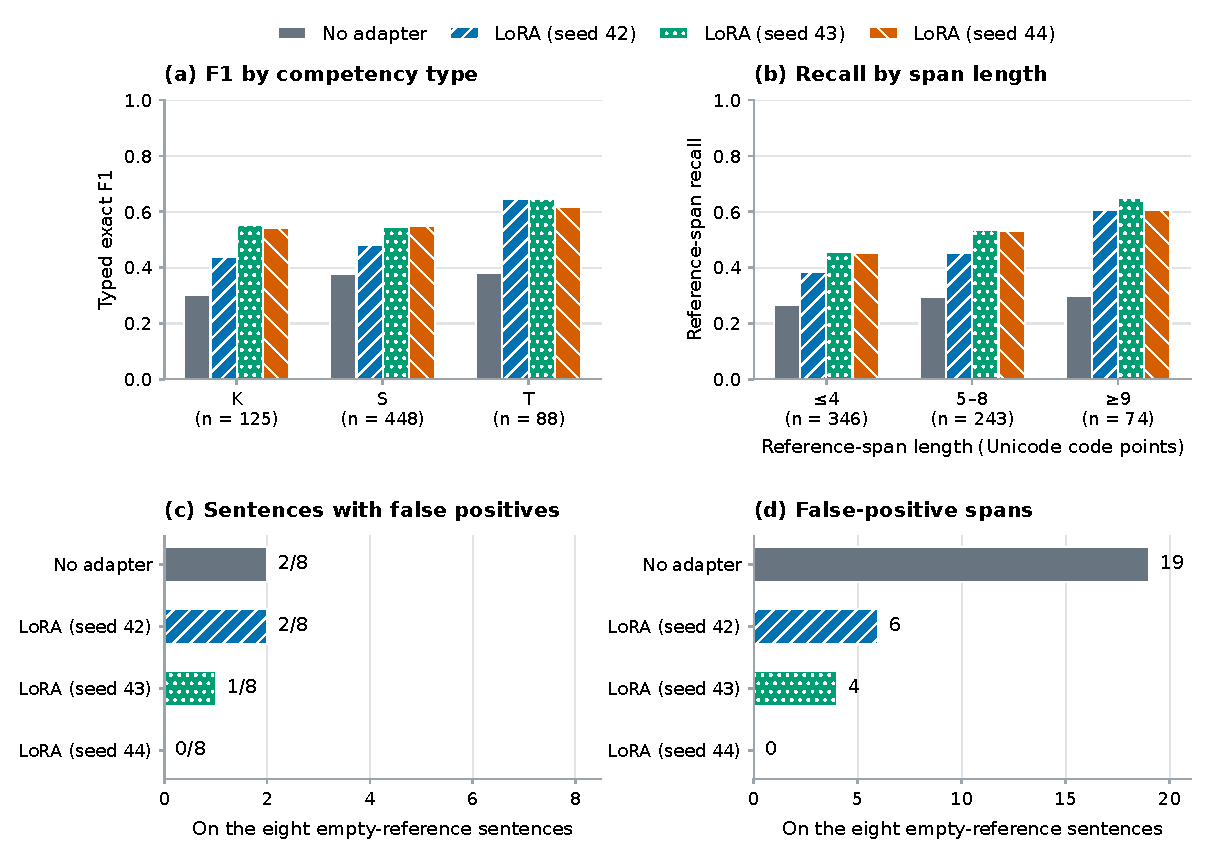
\includegraphics[width=\linewidth]{figures/qwen_diagnostics_chart_0913.pdf}
\caption{Qwen diagnostics on the human reference set: (a) typed exact-span F1 by type; (b) recall by reference-span length ($n$: reference spans); (c--d) false positives on eight sentences with no reference spans, counted by sentence and span.}
\label{fig:qwen-diagnostics}
\end{figure}


\subsection{Encoder and Competency-Type Comparisons}
\label{sec:external-benchmark-results}

XLM-R-large and ESCOXLM-R achieved mean typed exact-span micro-F1 scores of 0.522 and 0.538, respectively (Table~\ref{tab:external-chinese}, panel A). Scores were recomputed from all six archived prediction files against the same human reference set. The mean difference was 0.016, with a paired 95\% interval of $[-0.005, 0.035]$ (Table~\ref{tab:core-paired}). The interval includes zero and does not establish an advantage for ESCO initialization under this protocol.

Four-type macro-F1 was 0.607 for XLM-R-large and 0.622 for ESCOXLM-R. Averaging over K/S/T gave 0.542 and 0.562, respectively. These sensitivity summaries exclude the sparsely represented L category from the macro average without changing the four-type prediction task.

Qwen adaptation improved all three K/S/T categories (Table~\ref{tab:external-chinese}, panel B; Figure~\ref{fig:qwen-diagnostics}). The largest observed increase among these categories was for T, from 0.380 to 0.638. Mean S and K scores increased by 0.148 and 0.210, respectively. Among the three Silver-trained configurations in Table~\ref{tab:external-chinese}, panel B, Qwen had the highest observed mean scores for S and T, while ESCOXLM-R had the highest K score. These rankings are descriptive because prediction heads, training budgets, and inference procedures differ across architectures.

\begin{table}[!htbp]
\centering\small
\caption{Supervised adaptation of multilingual encoders on Gold150 (0--1), mean $\pm$ sample SD across three seeds.}
\label{tab:external-chinese}
\begin{tabularx}{\linewidth}{@{}Lrrrr@{}}
\toprule
Encoder & Typed exact & Typed relaxed & Boundary & Macro-F1 \\
\midrule
XLM-R-large & $0.522\pm0.022$ & $0.650\pm0.021$ & $0.571\pm0.022$ & $0.607\pm0.016$ \\
ESCOXLM-R & $0.538\pm0.021$ & $0.662\pm0.022$ & $0.582\pm0.024$ & $0.622\pm0.010$ \\
\bottomrule
\end{tabularx}
\par\smallskip\RaggedRight\footnotesize B2 training/development: 2,150/169 records. Fresh linear LSKT head; official \texttt{cnss-lskt-1.2.0} scorer; 150 human-reference records. Boundary is exact span matching with types collapsed; macro-F1 averages L/K/S/T. Gold150 is not a new blind test and contains only two L spans. All three seeds (42/43/44) are included; per-seed scores and selected epochs are retained in the model audit archive.
\end{table}

\begin{table}[!htbp]
\centering\small
\caption{Common-protocol typed exact token-span micro-F1 (0--1), mean $\pm$ sample SD across three seeds.}
\label{tab:external-common}
\begin{tabularx}{\linewidth}{@{}L P{.14\linewidth}P{.25\linewidth}rr@{}}
\toprule
Dataset & Stream & Train/dev/test & XLM-R-large & ESCOXLM-R \\
\midrule
SkillSpan & Skill & 4,800/3,174/3,569 & $0.567\pm0.012$ & $0.577\pm0.006$ \\
SkillSpan & Knowledge & 4,800/3,174/3,569 & $0.698\pm0.021$ & $0.672\pm0.052$ \\
Kompetencer & Skill & 778/346/262 & $0.545\pm0.028$ & $0.527\pm0.004$ \\
Kompetencer & Knowledge & 778/346/262 & $0.618\pm0.035$ & $0.593\pm0.044$ \\
Gnehm ICT & ICT & 19,889/2,332/2,557 & $0.891\pm0.005$ & $0.867\pm0.032$ \\
Green & Native types & 8,669/964/335 & $0.493\pm0.009$ & $0.492\pm0.007$ \\
Sayfullina & Skill & 3,705/1,855/1,851 & $0.920\pm0.004$ & $0.925\pm0.005$ \\
FIJO & Native types & 399/50/50 & $0.343\pm0.019$ & $0.339\pm0.007$ \\
\bottomrule
\end{tabularx}
\par\smallskip\RaggedRight\footnotesize Both encoders use fresh linear BIO heads, 20 epochs, and development-set checkpoint selection. SkillSpan and Kompetencer have separate skill and knowledge streams; Green and FIJO retain their entity types. German data use the public ICT release. The shared protocol differs from the original CRF and NNOSE methods.
\end{table}



\subsection{Boundary and Type Disagreements in Human Annotation}

The blinded annotation study found disagreement in both span boundaries and types. Mean boundary-only exact-span F1 was 0.850, compared with 0.818 when matching also required identical types (Table~\ref{tab:quality-main}). The decrease when type matching is required shows that type assignment contributes to disagreement beyond span boundaries.

The agreement study and model evaluation use different texts, label versions, and annotation procedures. Direct comparison of human and model agreement would require evaluating both on a common independently annotated sample.

\subsection{Scoring Criteria and Evaluation Targets}

For the same unadapted Qwen predictions, relaxing the matching criterion raises F1 from 0.361 to 0.470 (Table~\ref{tab:gold150-shared-r7}). Under typed exact matching, the 181 false positives comprise 27 same-boundary/different-type pairs, 89 same-type/overlapping-boundary pairs, and 65 other unmatched predictions. This grouping compares predicted boundaries and types with the reference annotations. A relaxed match still requires the same type and an IoU of at least 0.5.

Two unadapted Qwen outputs illustrate these distinctions. For \texttt{1801-s0004}, the prediction is the S span \zh{参与公司无人机飞控系统技术项目开发策划} (participate in planning a technical development project for the company's UAV flight-control system), whereas an overlapping reference S span is \zh{技术项目开发策划} (technical project development planning). Their overlap is below the relaxed threshold, so this pair matches under neither criterion. For \texttt{1802-s0005}, both layers select \zh{方法} (method), but the prediction is S and the reference is K. This pair has identical boundaries but fails both typed matching rules. Appendix~C gives the complete source sentences and offsets for these prediction--reference comparisons.

The exploratory expanded-pool Qwen runs produced different rankings across evaluation targets. With seed 42, the adopted expanded pool yielded F1 of 0.809 on its Silver test set and 0.585 on the shared human reference, whereas the alternative yielded 0.759 and 0.597, respectively (Table~\ref{tab:expanded-silver-main}). The adopted pool had the higher Silver-test score, and the alternative had the higher human-reference score. The pool-specific Silver tests differ in both texts and labels. The \hyperref[sec:annotation-quality]{annotation-quality analysis} provides the common-sentence comparison against blinded human annotations. Table~\ref{tab:source-stages} gives the constituent batches and final counts.

Exploratory expanded JobBERT results in Appendix~C show lower human-reference scores under jointly changed supervision, source composition, and model selection.
